\documentclass{book}
\usepackage[fontset=windows]{ctex} % 使用 Windows 内置字体集,已包含中文字体支持
\usepackage{graphicx}
\usepackage{amsmath}       % 数学公式增强宏包
\usepackage{physics}      % 物理符号宏包
\usepackage{amssymb}       % 数学符号宏包
\usepackage{bm}            % 用于加粗数学符号

\usepackage{geometry}      % 页面布局宏包
\geometry{a4paper, margin=1in} % 设置页面大小和边距
\usepackage{fancyhdr}      % 页眉页脚宏包
\pagestyle{fancy}
\fancyhead{}               % 清除默认页眉
\fancyfoot{}               % 清除默认页脚
\fancyhead[L]{高等量子力学笔记} % 左侧页眉
\fancyhead[R]{ZhangX}     % 右侧页眉
\fancyfoot[C]{\thepage}   % 中间页脚显示页码
\usepackage{listings}      % 代码高亮宏包
\usepackage{xcolor}        % 颜色宏包
\lstset{                    % 设置代码高亮样式
    backgroundcolor=\color{lightgray!20}, % 背景颜色
    basicstyle=\ttfamily,   % 基本字体
    keywordstyle=\color{blue}, % 关键词颜色
    commentstyle=\color{green!50!black}, % 注释颜色
    stringstyle=\color{red}, % 字符串颜色
    numbers=left,           % 行号位置
    numberstyle=\tiny\color{gray}, % 行号样式
    stepnumber=1,          % 行号步长
    numbersep=5pt,         % 行号与代码间距
    showstringspaces=false, % 不显示字符串中的空格
    breaklines=true,       % 自动换行
    frame=single,          % 代码框
    tabsize=4,             % Tab 键宽度
    captionpos=b           % 标题位置
}
% \usepackage{unicode-math}  % Unicode 数学字体支持
% \setmathfont{Latin Modern Math} % 设置数学字体

\usepackage{bookmark}      % 先加载 bookmark
\usepackage{hyperref}      % 后加载 hyperref
\hypersetup{
    colorlinks=true,
    linkcolor=blue,
    bookmarksopen=true,
    pdfauthor={ZhangX},
    pdftitle={高等量子力学笔记}
}

\newenvironment{abstract}{\section*{README}}{\par}
\title{高等量子力学笔记}
\author{ZhangX}
\date{\today} % 自动插入当前日期

\begin{document}
\maketitle

\begin{abstract}
本文是作者基于《现代量子力学(第二版)》 (by 樱井纯)学习过程所记录的笔记。
\end{abstract}


\chapter{基本概念} % 中文章节标题
《现代量子力学(第二版)》这本书摒弃了初等量子力学中按照历史发展顺序对量子力学一点一点介绍,而是从一个打破传统认知的实验开始。
\section{斯特恩-盖拉赫实验}
斯特恩-盖拉赫实验的前提认知是银原子中一个电子($5s$)的自旋(内禀的)提供了整个原子的磁矩,于是整个原子的磁矩满足,
\begin{equation}
    \bm{\mu} \propto \mathbf{S}
    \label{eq:1.1}
\end{equation}
其中,比例因子为 $\displaystyle \frac{e}{m_ec}$ 。磁矩在外加的磁场中会发生偏转。相互作用能为 $-\bm{\mu} \cdot \mathbf{B}$ ,
于是受力在 $z$ 方向分量的大小为
\begin{equation}
    F_z = \frac{\partial}{\partial z}\left(\bm{\mu}\cdot\mathbf{B}\right) 
    \simeq \mu_z \frac{\partial B_z}{\partial z}
    \label{eq:1.2}
\end{equation}
于是这个实验设计了一个局部不均匀磁场,这也是这个实验中创新的地方。按照经典力学的观点,原子取向是任意的,
那么 $\bm{\mu}$ 便无取向偏好,那 $\mu_z$ 便可以在 $[-|\bm{\mu}|, |\bm{\mu}|]$ 之间连续取值。形成一个弥散的斑痕,然而,事实并不如人们想的那样。
\begin{figure}[h]
    \centering
    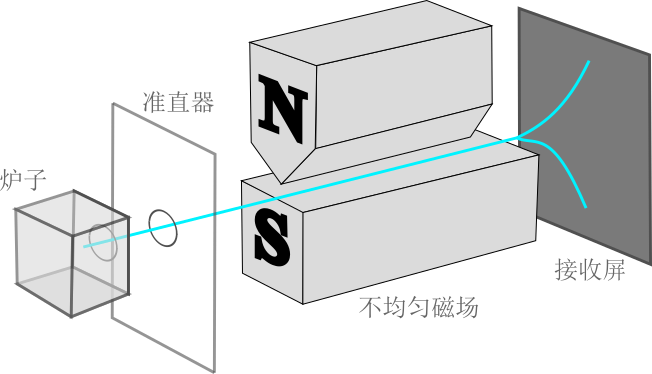
\includegraphics[width=0.5\textwidth]{img/斯特恩}
    \caption{Stern-Gerlach 实验}
    \label{fig:1.1}
\end{figure} 
实验的结果是如图 ~\ref{fig:1.1} 所示的两个点状图样。这就是空间量子化的宏观表现。然后我们设计进一步的实验,
\subsection{序列斯特恩-盖拉赫实验}
这一部分暂时不写,懒~

\section{右矢、左矢和算符}
狄拉克发明的右矢(Ket)和左矢(Bra)符号体系,为量子力学的计算提供了简洁的数学框架。 
\subsection{右矢空间}
为什么人们对于量子世界难以理解,就在于量子世界和经典世界对于物理量的描述方式是完全不同的。
在量子世界大门被推开的那一刻,人们是懵逼的,他们无法理解为什么一个粒子可以同时处在A和B两个位置上(实际并不是同时处于两个位置上,
只是两个位置上都有可能被测量到)。
随着实验和理论的推进,人们才意识到,量子是以概率幅存在的,那么就无法用一个数值去对其进行描述了。
那我们怎么描述,很简单,我们就用一个盒子把不同位置的概率幅装起来,然后有人问的时候,我们就把这个盒子打开给他看。
除了装位置的盒子,我们还有装动量的盒子,装能量的盒子,装自旋的盒子等等,然后我们把所有的盒子都放在一个大的盒子里。
这样就能完备的描述一个量子系统。这个盒子就是狄拉克定义的一个右矢$|\psi\rangle$。其中由于需要满足归一化的要求,
所以 $|\alpha\rangle$ 和 $c|\alpha\rangle$ (c为任意非零复数)描述的是同一个量子态。

\subsection{左矢空间和内积}
左矢空间和右矢空间相互对偶,且一一映射,用 $\langle \alpha |$ 表示,左矢空间由本征左矢张成,与右矢空间的一一对应关系写为
\begin{equation}
    \langle \alpha| \overset{DC}{\longleftrightarrow } |\alpha\rangle
    \label{eq:1.4} 
\end{equation}
其中, $DC$ 代表对偶映射(Dual Correspondence)。
左矢和右矢之间可以定义内积 $\langle \beta | \alpha \rangle$,其结果为一个复数,且与 $\langle \alpha | \beta \rangle$ 互为复共轭。记为:
\begin{equation}
    \langle \beta | \alpha \rangle = \langle \alpha | \beta \rangle^*
    \label{eq:1.5} 
\end{equation}

\subsection{算符}
一个算符代表了一种观测,可以将一个右矢映射到另一个右矢上,也许这个新的右矢的盒子中装的东西是不同的。当盒子里的东西保持不变时。
我们把这个盒子叫做这个算符的本征右矢,又叫本征态。例如,自旋的例子:
\begin{equation}
    \hat{S}_z |\hat{S}_z; +\rangle = \frac{\hbar}{2} |\hat{S}_z; +\rangle, 
    \hat{S}_z |\hat{S}_z; -\rangle = -\frac{\hbar}{2} |\hat{S}_z; -\rangle
    \label{eq:1.3}
\end{equation}

现在我们考虑
% \\
% \\下面是AI生成的内容,我注释掉了,后面可能会参考然后做修改
% 量子力学中,系统的量子态由希尔伯特空间(Hilbert Space)中的右矢(记为 $|\psi\rangle$)描述。希尔伯特空间是一个完备的内积线性空间,其元素(右矢)是“概率幅”的集合——这与经典物理中用确定数值描述物理量的方式截然不同。  

% 在经典世界中,粒子的位置是确定的(例如“在A点”或“在B点”);但在量子世界中,粒子的状态是叠加态(Superposition)。例如,一个粒子的位置态可表示为:  
% $$
% |\psi\rangle = c_A |\mathbf{r}_A\rangle + c_B |\mathbf{r}_B\rangle
% $$  
% 其中 $|\mathbf{r}_A\rangle$ 和 $|\mathbf{r}_B\rangle$ 是位置本征态(分别对应“在A点”和“在B点”),$c_A, c_B$ 是复数概率幅(满足归一化条件 $|c_A|^2 + |c_B|^2 = 1$)。  

% 叠加态的本质是:测量时会坍缩到某一确定的位置本征态(如 $|\mathbf{r}_A\rangle$ 或 $|\mathbf{r}_B\rangle$),其概率由概率幅的模平方决定($|c_A|^2$ 或 $|c_B|^2$)。为了直观描述这种概率分布,我们可以将右矢 $|\psi\rangle$ 类比为“盒子”——它包含了所有可能的测量结果的概率幅信息;当需要具体计算时(如测量位置),我们将“盒子”投影到位置表象,得到波函数 $\psi(\mathbf{r}) = \langle \mathbf{r} | \psi \rangle$(即位置概率幅),其模平方 $|\psi(\mathbf{r})|^2$ 就是粒子在 $\mathbf{r}$ 处的概率密度。  

% 左矢(记为 $\langle \phi |$)是右矢空间的对偶空间元素,用于定义内积运算。内积 $\langle \phi | \psi \rangle$ 是一个复数,其模平方 $|\langle \phi | \psi \rangle|^2$ 表示“在态 $|\phi\rangle$ 中测量到态 $|\psi\rangle$ 的概率”。在位置表象下,左矢 $\langle \mathbf{r} |$ 与右矢 $|\psi\rangle$ 的内积即为波函数 $\psi(\mathbf{r})$,这是连接抽象右矢与具体物理测量的关键桥梁。


\subsubsection{定义及运算法则}
可行的运算
\begin{itemize}
    \item c $|\alpha \rangle = |\alpha \rangle c$,c为复数
    \item $|\alpha \rangle + |\beta\rangle$
\end{itemize}








\end{document}